\documentclass[10pt,a4paper,twocolumn]{article}
\usepackage[left=17mm,right=17mm,top=21mm,bottom=22mm,headheight=12pt,headsep=14pt,footskip=25pt]{geometry}
\usepackage{amsmath}
\usepackage{fontspec,unicode-math}
\setmainfont{texgyretermes-regular.otf}[
  BoldFont=texgyretermes-bold.otf,
  ItalicFont=texgyretermes-italic.otf,
  BoldItalicFont=texgyretermes-bolditalic.otf,
]
\setmathfont{texgyretermes-math.otf}
\usepackage[table]{xcolor}
\usepackage{graphicx}
\usepackage{booktabs,tabularx,array}
\usepackage{titlesec,fancyhdr,microtype,balance}
\usepackage[super,sort&compress]{natbib}
\usepackage[font=small,labelfont=bf,labelsep=period,justification=justified,singlelinecheck=false]{caption}
\usepackage{tikz}
\usetikzlibrary{arrows.meta,positioning}
\usepackage{xurl}
\usepackage[colorlinks=true,linkcolor=LinkBlue,citecolor=LinkBlue,urlcolor=LinkBlue,pdfauthor={Shodh AI Research},pdftitle={Beyond reconstruction error: falsification tests for scientific representations}]{hyperref}

\definecolor{LinkBlue}{HTML}{13468B}
\definecolor{NCBlue}{HTML}{00659A}
\definecolor{NCInk}{HTML}{132430}
\definecolor{NCGray}{HTML}{EEF2F4}
\definecolor{NCPaleBlue}{HTML}{E3EFF8}
\definecolor{NCPaleAmber}{HTML}{FFF0D5}
\definecolor{NCPaleGreen}{HTML}{E4F1E8}
\setlength{\columnsep}{16pt}
\setlength{\parindent}{10pt}
\setlength{\parskip}{0pt}
\setlength{\emergencystretch}{1.3em}
\setlength{\dbltextfloatsep}{10pt plus 3pt minus 2pt}
\setlength{\textfloatsep}{9pt plus 3pt minus 2pt}
\setlength{\abovecaptionskip}{5pt}
\setcounter{dbltopnumber}{2}
\renewcommand{\dbltopfraction}{0.78}
\widowpenalty=10000
\clubpenalty=10000
\renewcommand\figurename{Fig.}
\DeclareCaptionLabelSeparator{bar}{\enspace|\enspace}
\captionsetup{labelsep=bar,font=footnotesize}
\titleformat{\section}{\normalfont\bfseries\fontsize{12}{14}\selectfont}{\thesection}{0.6em}{}
\titleformat{\subsection}[hang]{\normalfont\bfseries\fontsize{11}{13}\selectfont}{\thesubsection}{0.6em}{}
\titlespacing*{\section}{0pt}{10pt plus 2pt}{4pt}
\titlespacing*{\subsection}{0pt}{7pt plus 2pt}{3pt}
\setcounter{secnumdepth}{2}
\makeatletter
\renewcommand\@biblabel[1]{#1.}
\makeatother
\pagestyle{fancy}
\fancyhf{}
\fancyhead[L]{\footnotesize\itshape Beyond reconstruction error}
\fancyhead[R]{\footnotesize\itshape Shodh AI Research}
\fancyfoot[C]{\footnotesize\thepage}
\renewcommand{\headrulewidth}{0.4pt}
\renewcommand{\footrulewidth}{0pt}
\fancypagestyle{first}{\fancyhead{}\renewcommand{\headrulewidth}{0pt}}
\newcolumntype{Y}{>{\raggedright\arraybackslash}X}
\newcolumntype{P}[1]{>{\raggedright\arraybackslash}p{#1}}
\newcommand{\gate}[1]{\text{\textbf{#1}}}
\newcommand{\doilink}[1]{\href{https://doi.org/#1}{doi:#1}}
\tikzset{
  flow/.style={draw=NCInk!75,thick,rounded corners=2pt,align=center,
    font=\sffamily\footnotesize,inner sep=5pt,minimum height=10mm,fill=NCGray},
  wire/.style={-{Latex[length=2mm]},semithick,draw=NCInk},
  lab/.style={font=\sffamily\bfseries\small,anchor=west},
  note/.style={font=\sffamily\scriptsize,align=center,text=NCInk},
  mini/.style={flow,minimum height=7mm,font=\sffamily\scriptsize,inner sep=3pt},
}

\begin{document}
\twocolumn[{
\vspace*{5pt}
\begin{center}
{\bfseries\fontsize{19}{24}\selectfont
Beyond Reconstruction Error:\\
Falsification Tests for Scientific Representations\par}
\vspace{7pt}
{\fontsize{12}{14}\selectfont Shodh AI Research\par}
\vspace{3pt}
{\small Preprint\enspace\textperiodcentered\enspace 28 November 2026\par}
\end{center}
\vspace{6pt}
\hrule height 0.4pt
\vspace{6pt}
\noindent{\bfseries\fontsize{12}{14}\selectfont Abstract}\par
\vspace{2pt}
\noindent
Scientific representations can reconstruct selected values accurately while losing information or physical properties required by a scientific claim. We introduce fail-closed validation, which binds each claim to a population, lawful transformations, physical quantities, a total stored-byte budget, frozen thresholds and reference evidence. The validator returns \gate{PASS}, \gate{FAIL} or \gate{ABSTAIN}. A seven-system retrospective audit, supported by a screen of 1,211 pull requests, identified failures involving objective substitution, physical parity, split ancestry, metric denominators and evidence custody. In a recovered paired experiment, the held-out normalized objective fell by 96.98\%, yet both frozen raw-unit superiority gates failed. In cylindrical flow, a fixed-order operator replay was bitwise reproducible while a separate physical trajectory exceeded its radial error gate. An archived single-shock comparison reports lower reconstruction error for two external codecs than for the frozen learned representation. In the sealed benchmark of 160 physical units, fail-closed validation rejected 4,186 of 4,320 prescribed mutant variants, compared with 2,055 for reconstruction alone. It abstained on 640 of 640 withheld-evidence controls.\par
\vspace{4pt}
\noindent{\small\textbf{Keywords:} scientific representations; reconstruction error; falsification; data compression; physical diagnostics; provenance\par}
\vspace{12pt}
\hrule height 0.4pt
\vspace{4pt}
}]
\thispagestyle{first}
\section{Introduction}

Scientific machine learning uses compact representations for storage, simulation, and design. Reconstruction error measures the distance between a target and a decoded state under a particular evaluation path. A representation used for scientific inference may also need to preserve a conservation law, distinguish physically different states, or generalize across independent simulations. A single reconstruction score leaves these requirements untested.

\textbf{Shortcut learning and evaluation leakage.}
Geirhos et al.\ describe shortcuts that solve the training objective by exploiting cues that do not support the intended task.\cite{geirhos} Lapuschkin et al.\ demonstrate how strong scores can coexist with such cues,\cite{lapuschkin} and Kapoor and Narayanan document the consequences of leakage in scientific applications.\cite{kapoor} A representation can exploit a more direct route: auxiliary inputs to the decoder may contain information assigned to the latent code. Similarly, distinct file names do not establish independence when their contents descend from the same simulations. Similarity-aware splitting and blocked cross-validation address related forms of dependence,\cite{datasail,roberts} while work on reusable holdouts addresses the effect of adaptive selection.\cite{dwork} Datasheets and model cards document scope, provenance and intended uses.\cite{gebru,mitchell} Our claim cards make selected obligations executable and link them to decisions and retained evidence.

\textbf{Scientific benchmarks and matched baselines.}
PDEBench, the extensible simulation benchmark of Otness et al., and The Well provide controlled simulation datasets and baseline protocols.\cite{pdebench,otness,well} McGreivy and Hakim show how weak baselines and selective reporting inflate apparent gains in fluid-related PDE studies.\cite{mcgreivy} Studies of physics-informed networks identify optimization failures and imbalanced gradients in objectives that include physical residuals.\cite{krishna,wang} These findings motivate paired controls, original-unit comparisons and quantity-specific errors when an objective improves.

\textbf{Invariance, reconstruction and scientific compression.}
SLICES encodes crystal connectivity across periodic cells, whereas CDVAE models periodic structures with a diffusion decoder and Mat2Seq constructs invariant crystal sequences.\cite{xiao,xie,yan} These approaches illustrate that invariance and geometric recovery are separate properties. Frame averaging provides a route to equivariance, and continuity results delimit when canonicalization is available.\cite{puny,dym} Matbench and Matbench Discovery distinguish property prediction and stability screening from reconstruction.\cite{dunn,riebesell} In simulation compression, ZFP, SZ and SZ3 provide controlled distortion, and TTHRESH exploits multidimensional tensor structure.\cite{lindstrom,sz2018,sz3,tthresh} Work on gyrokinetic plasma compression demonstrates the need for structural and spatiotemporal diagnostics alongside distortion.\cite{galletti} We compare codecs under a common ceiling on actual stored bytes and evaluate physical errors separately from reconstruction.

\textbf{Verification and falsification.}
Scientific verification and validation distinguish numerical correctness from adequacy for a physical application.\cite{yeo,asme} Metamorphic tests assess a computation through relations between transformed inputs and outputs. Mutation testing measures whether an evaluation can reject deliberately defective artifacts.\cite{lin,jia} We bring these ideas together in a procedure that tests specific claims, reports false rejection on lawful controls, and abstains when required evidence is unavailable.

This work makes three contributions. First, it specifies an architecture for evaluating stored representations against a frozen scientific claim (Fig.~\ref{fig:architecture}). Second, it traces failures from a favorable headline metric to an observation that changed the scientific decision. Third, it specifies a public protocol that compares reconstruction-only and fail-closed validators on the same controlled defects and reports coverage at declared byte ceilings.

\section{Results}

\subsection{A normalized objective improved while raw-unit comparisons failed}
We reviewed seven scientific machine learning and simulation workstreams. The evidence unit was a documented claim and its associated control. The repository screen counted 1,100 records in one repository and 111 in the other. A reconstruction of the first inventory from dated pull request metadata matches the archived totals, including 758 open, 361 merged and 92 closed without merge across both repositories. These records were leads for identifying mechanisms. Several records can describe the same experiment.

In the biomolecular interaction case, a paired optimization ladder compared a group-balanced normalized objective with a frozen control at 1, 4, 16 and 64 steps. The recovered 64-step result records a held-out normalized loss reduction of 0.9698438. The candidate failed both frozen raw-unit gates: it did not beat the paired raw-unit control or the training-location predictor. The archived run and its evidence seal retain the rejection without replacing the final rung.

\begin{figure*}[t]
\centering
\resizebox{\textwidth}{!}{%
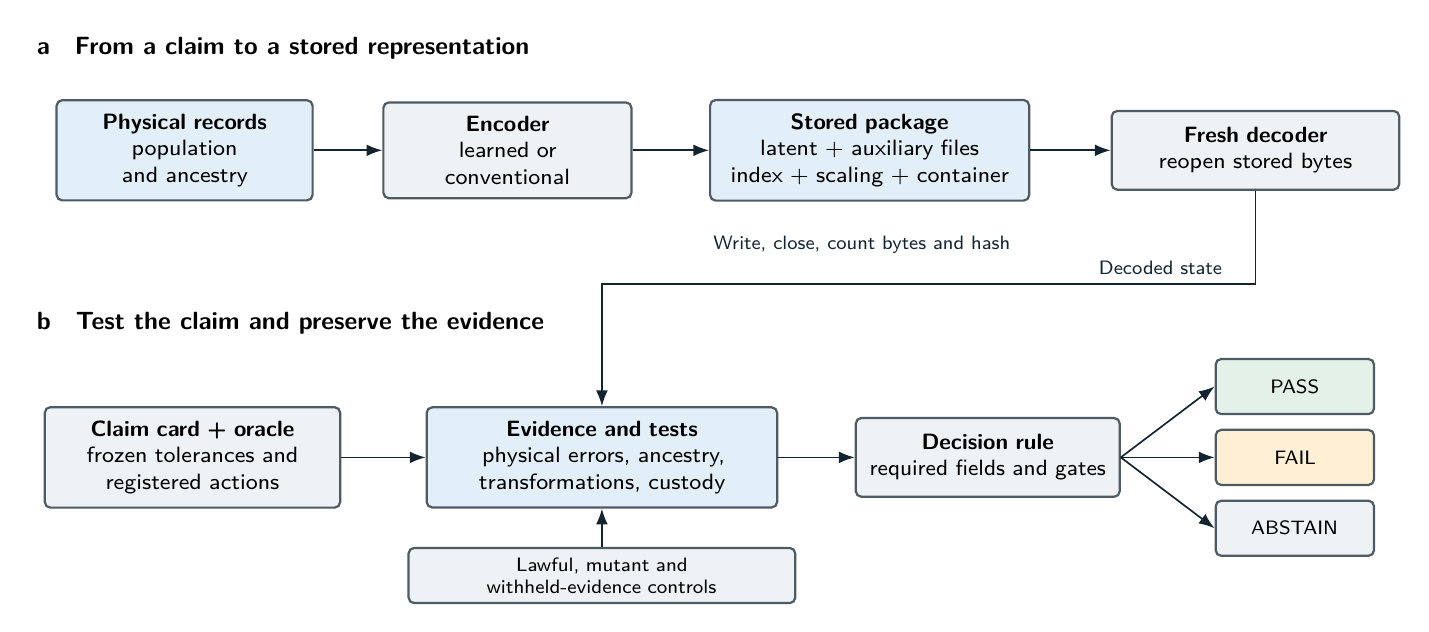
\begin{tikzpicture}[x=1mm,y=1mm]
  \node[lab] at (0,0) {a\quad From a claim to a stored representation};
  \node[flow,text width=29mm,fill=NCPaleBlue] (pop) at (20,-13)
    {\textbf{Physical records}\\population and ancestry};
  \node[flow,text width=28mm] (encoder) at (61,-13)
    {\textbf{Encoder}\\learned or conventional};
  \node[flow,text width=37mm,fill=NCPaleBlue] (bytes) at (107,-13)
    {\textbf{Stored package}\\latent + auxiliary files\\index + scaling + container};
  \node[flow,text width=33mm] (decode) at (156,-13)
    {\textbf{Fresh decoder}\\reopen stored bytes};
  \draw[wire] (pop)--(encoder); \draw[wire] (encoder)--(bytes);
  \draw[wire] (bytes)--(decode);
  \node[note] at (106,-25) {Write, close, count bytes and hash};
  \node[lab] at (0,-35) {b\quad Test the claim and preserve the evidence};
  \node[flow,text width=34mm] (oracle) at (21,-52)
    {\textbf{Claim card + oracle}\\frozen tolerances and\\registered actions};
  \node[flow,text width=41mm,fill=NCPaleBlue] (tests) at (73,-52)
    {\textbf{Evidence and tests}\\physical errors, ancestry,\\transformations, custody};
  \node[flow,text width=30mm] (verdict) at (122,-52)
    {\textbf{Decision rule}\\required fields and gates};
  \node[mini,fill=NCPaleGreen,text width=18mm] (pass) at (161,-43) {PASS};
  \node[mini,fill=NCPaleAmber,text width=18mm] (fail) at (161,-52) {FAIL};
  \node[mini,fill=NCGray,text width=18mm] (abstain) at (161,-61) {ABSTAIN};
  \draw[wire] (oracle)--(tests); \draw[wire] (tests)--(verdict);
  \draw[wire] (decode.south) -- (156,-30) -- (73,-30) -- (tests.north);
  \node[note,anchor=south east] at (153,-30) {Decoded state};
  \draw[wire] (verdict.east)--(pass.west);
  \draw[wire] (verdict.east)--(fail.west);
  \draw[wire] (verdict.east)--(abstain.west);
  \node[mini,text width=47mm] (controls) at (73,-67)
    {Lawful, mutant and withheld-evidence controls};
  \draw[wire] (controls)--(tests);
\end{tikzpicture}%
}
\caption{\textbf{Fail-closed validation architecture.} \textbf{a,} The encoder produces a stored representation. The decoder opens the closed package in a fresh process and can use only the declared auxiliary bytes. \textbf{b,} Each result is evaluated against a frozen claim card and reference. Lawful controls measure false rejection, mutants measure detection, and deliberately withheld inputs test abstention.}
\label{fig:architecture}
\end{figure*}

\subsection{Reproducibility and physical parity required separate checks}
In the cylindrical Couette case, a retained fixed contributor-order spread produced bitwise-identical results across fresh processes. A separate strict one-step test reproduced its retained population arrays. In the ordinary trajectory replay, the A and B arrays differed. The frozen bulk radial relative-$L_2$ error was 0.050419, beyond the 0.05 acceptance threshold. A separately formulated body-fitted calculation produced approximately $3.32\times10^{-6}$ on the corresponding radial metric. Its incompressible formulation provides an independent comparison with a narrower interpretation than solver identity.

Per-step host capture shifted the axial relative-$L_2$ metric beyond both two-replicate envelopes in an interleaved A--B--B--A design. Final-only capture had the same gate vectors across the four processes and no metric separated the envelopes. The recovered manifests and readbacks support these two scoped observations. They do not resolve whether a smaller effect exists outside the measured panel.

\subsection{Ancestry and metric scaling changed the interpretation}
In the fracture workstream, the historical registry and development reports describe two nominal holdouts as reruns of the same 128 parent simulations. The archived record supports a single surrogate-damage evaluation cohort. The full sample-to-parent mapping and exact historical checkpoint roots remain unavailable for independent reproduction.

An arithmetic control isolates normalization. For the target $[100,102]$ and prediction $[100.2,102.2]$, the target-norm relative-$L_2$ error is 0.0019801, while the RMSE divided by the target's population standard deviation is 0.2. The latter fails a threshold of 0.10. The offset and the threshold define a demonstration of denominator sensitivity, without an estimate of its frequency in scientific data.

\subsection{Evidence custody and engine semantics limited the verdict}
The recovered molecular dynamics panels compared JAX and GROMACS endpoints for the same initial state at three time steps, with 14 checks per row. An earlier rounded-box comparison passed 39 of 42 checks and failed the box check in every row. After full-precision box extraction, all 42 checks passed at a 0.020\,ps horizon. A separate 0.080\,ps panel also passed all 42 checks on that initial state. These are bounded endpoint comparisons. A recovered follow-up log records a failed wrapper hash check against a scheduler spool path. Historical records also identify a parser assumption that treated molecule-template masses as a globally expanded atom table. That follow-up did not establish a scientific verdict for its intended comparison.

A differentiable molecular simulator passed bounded native consistency checks, including a one-step run with 93 of 93 bonds in bounds. The available evidence does not include all-particle force, world-frame torque and energy-component parity against an external engine. In a separate field workstream, initialized full-size forward and vector--Jacobian product checks exercised the implementation. Learned fidelity requires a trained candidate and an independent evaluation.

The wider records also contained reports of transform and boundary mismatches, residuals satisfied by construction, unmatched reference domains, obsolete contracts, source checks without native parity, and engineering tests despite failed convergence. We use these records to define failure mechanisms. Several original case artifacts still need independent replay.

\subsection{External codecs changed the single-trajectory comparison}
An archived aerodynamic pilot compared a frozen learned representation with six comparators on one held-out perturbed normal-shock trajectory. Under a declared 2,097,152-byte payload ceiling, the archived metrics rank SZ3 and TTHRESH ahead of the frozen representation (Table~\ref{tab:shock}). The recovered input array matches the original dataset manifest by SHA-256. The original metrics JSON and payload manifest remain inaccessible, so the quoted values are attributed to the retained run report. The public codec benchmark uses a separate population and protocol.

\begin{table}[!t]
\caption{\textbf{Archived single-trajectory compression pilot.} Lower mean active-channel $z$-RMSE is better. The original metrics and payload files remain unavailable for revalidation.}
\label{tab:shock}
\centering\small
\begin{tabularx}{\columnwidth}{@{}Yr@{}}
\toprule
Method & $z$-RMSE\\
\midrule
SZ3 & 0.007035\\
TTHRESH & 0.011368\\
Tucker-only & 0.038367\\
Frozen learned representation & 0.077538\\
POD/SVD & 0.097413\\
ZFP & 0.269694\\
Eight-step neural diagnostic & 0.631845\\
\bottomrule
\end{tabularx}
\end{table}

The ZFP format floor was reported as 2,101,248 bytes, 4,096 bytes above the ceiling. The eight-step neural diagnostic was deliberately under-trained. The pilot lacks authoritative meshes, surface registration and per-sample boundary-condition graphs for a geometry-aware comparison. Its scope is one trajectory and its declared accounting rule.

\subsection{Public benchmark preparation and calibration}
The public benchmark manifest contains 256 periodic compressible flow trajectories and 256 bulk crystal structures. Each module has 128 training groups, 48 validation groups and 80 reporting groups, with each physical parent assigned to one partition (Fig.~\ref{fig:benchmark}). The selected units passed manifest and ancestry checks. SZ3, ZFP and TTHRESH encoded a PDEBench training trajectory and decoded the stored artifacts in separate processes. The calibration run evaluated 240 lawful controls per module and froze the resulting claim cards on the validation partition.

All three seeds completed on H100 GPUs. Five of the six module-by-seed runs met the predefined validation plateau criterion. Grid seed 41 reached the 450-epoch cap without meeting it (Fig.~\ref{fig:training}). These validation results describe training and checkpoint selection. The reporting results below use the separate sealed split.

\begin{figure*}[t]
\centering
\resizebox{\textwidth}{!}{%
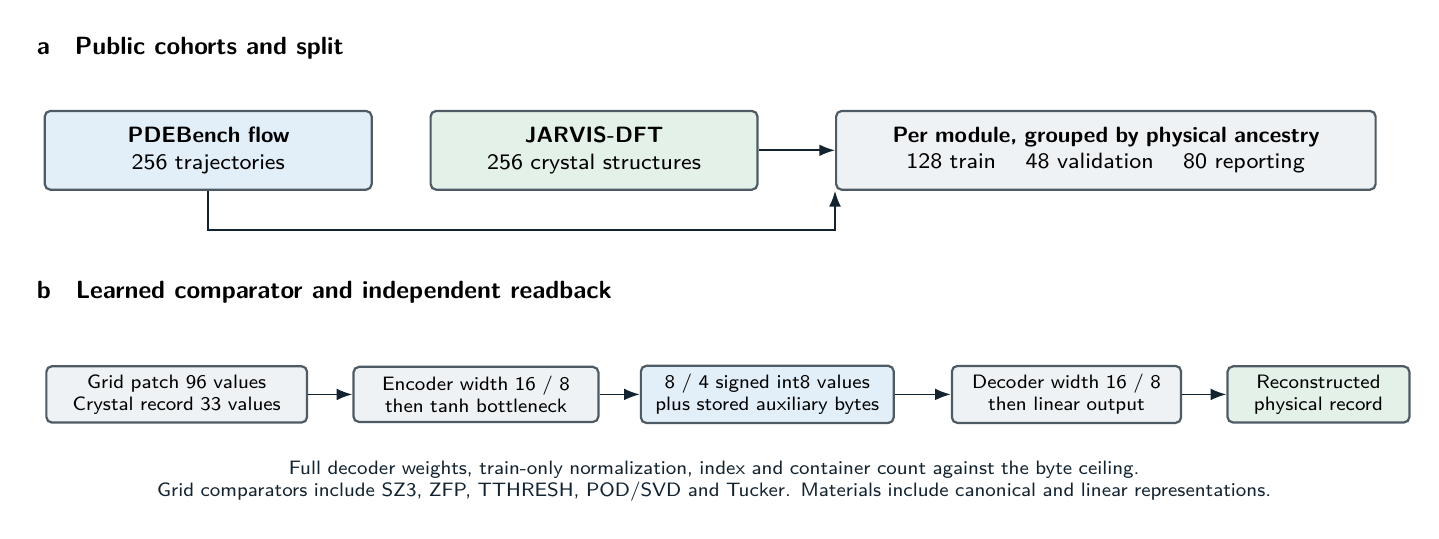
\begin{tikzpicture}[x=1mm,y=1mm]
  \node[lab] at (0,0) {a\quad Public cohorts and split};
  \node[flow,text width=38mm,fill=NCPaleBlue] (g) at (23,-13)
    {\textbf{PDEBench flow}\\256 trajectories};
  \node[flow,text width=38mm,fill=NCPaleGreen] (m) at (72,-13)
    {\textbf{JARVIS-DFT}\\256 crystal structures};
  \node[flow,text width=65mm] (s) at (137,-13)
    {\textbf{Per module, grouped by physical ancestry}\\128 train \quad 48 validation \quad 80 reporting};
  \draw[wire] (m)--(s);
  \draw[wire] (g.south) -- ++(0,-5) -| (s.south west);
  \node[lab] at (0,-31) {b\quad Learned comparator and independent readback};
  \node[mini,text width=31mm] (in) at (19,-44) {Grid patch 96 values\\Crystal record 33 values};
  \node[mini,text width=29mm] (e) at (57,-44) {Encoder width 16 / 8\\then tanh bottleneck};
  \node[mini,text width=30mm,fill=NCPaleBlue] (latent) at (94,-44)
    {8 / 4 signed int8 values\\plus stored auxiliary bytes};
  \node[mini,text width=27mm] (d) at (132,-44) {Decoder width 16 / 8\\then linear output};
  \node[mini,text width=21mm,fill=NCPaleGreen] (out) at (164,-44) {Reconstructed\\physical record};
  \draw[wire] (in)--(e); \draw[wire] (e)--(latent); \draw[wire] (latent)--(d); \draw[wire] (d)--(out);
  \node[note,text width=148mm] at (87,-55)
    {Full decoder weights, train-only normalization, index and container count against the byte ceiling.\\
    Grid comparators include SZ3, ZFP, TTHRESH, POD/SVD and Tucker. Materials include canonical and linear representations.};
\end{tikzpicture}%
}
\caption{\textbf{Public benchmark cohorts and learned baseline.} \textbf{a,} The flow trajectory and reduced-composition crystal groups each contribute one independent unit. All observations descended from a unit are kept in the same split. \textbf{b,} The first number describes the grid module and the second the crystal module. The network is trained separately for each module and seed. The evaluation passes only a closed package to a fresh decoder.}
\label{fig:benchmark}
\end{figure*}

\begin{figure*}[t]
\centering
\includegraphics[width=\textwidth]{figures/validation_loss.pdf}
\caption{\textbf{Validation traces for the three H100 training seeds.} \textbf{a,} Grid patch autoencoders on compressible-flow validation records. The vertical axis is logarithmic. \textbf{b,} Periodic crystal autoencoders evaluated in their normalized coordinates. Filled circles mark runs that met the plateau criterion, and an open square marks the grid run that reached the epoch cap. Losses were computed on validation data before sealed reporting.}
\label{fig:training}
\end{figure*}

\subsection{Sealed controls measured detection, false rejection and abstention}
The sealed evaluation completed for 160 physical units. The fail-closed evaluator detected more mutants in 30 of 54 module--family--severity cells and tied the reconstruction-only gate in 24 cells. Fig.~\ref{fig:detection} reports physical-unit bootstrap intervals and the variation across families. Table~\ref{tab:sealed-controls} gives counts and lawful false-rejection estimates. The pooled false-rejection estimate was 2.50\% (1.50\%--3.63\%) (95\% interval), compared with 4 of 800 lawful cases rejected by the in-memory RMSE gate. These comparisons measure response to the declared interventions. Several control families provide evidence flags computed from a known perturbation. In compressible flow, false rejection implicated relative-$L_2$ (4), boundary error (3), fluctuation-normalized RMSE (3), RMSE (3), tail error (3), divergence error (2), energy drift (2), mass drift (1), momentum drift (1), gradient error (1). An outcome can implicate more than one gate. In periodic crystals, false rejection implicated cell Gram (3), volume (3), RMSE (1), relative-$L_2$ (1). Of 134 passing information and observer variants, 133 had zero in-memory reconstruction error. The denominator retains these prescribed variants, including interventions that did not change any stored value. All gate reasons and per-unit verdicts are retained in the source data.

Across both modules, identity, independent-process, lawful-transformation and alternative-encoding controls together had 0/640 (0.0\%) false rejections. All false rejections arose in benign half-precision conversion: compressible flow had 15/80 (18.75\%; 95\% CI 10.00\%--27.50\%), and periodic crystals had 5/80 (6.25\%; 95\% CI 1.25\%--12.50\%). Pooled across lawful controls, this is 20/800 (2.50\%). Supplementary Table~1 gives the complete control-type breakdown and per-gate lawful retention; Supplementary Table~4 resolves abstention by omitted evidence field.

\begin{table*}[t]
\caption{\textbf{Decisions on the sealed control suite.} Mutant and withheld counts aggregate over control variants. False-rejection intervals resample physical units.}
\label{tab:sealed-controls}
\small
\begin{tabularx}{\textwidth}{@{}Yrrrrr@{}}
\toprule
Module & Units & RMSE detects & Fail-closed detects & Lawful FRR (95\% CI) & Withheld abstains\\
\midrule
Compressible flow & 80 & 1,112/2,160 & 2,160/2,160 & 3.75\% (2.00\%--5.50\%) & 320/320\\
Periodic crystals & 80 & 943/2,160 & 2,026/2,160 & 1.25\% (0.25\%--2.50\%) & 320/320\\
\bottomrule
\end{tabularx}
\end{table*}

\begin{figure*}[t]
\centering
\includegraphics[width=\textwidth,height=0.76\textheight,keepaspectratio]{figures/mutant_detection.pdf}
\caption{\textbf{Mutant detection on the reporting units.} Points summarize the fraction of prescribed mutant variants rejected by the in-memory reconstruction gate or the fail-closed evaluator. Error bars represent 95\% bootstrap intervals over physical units. The side-information variants share the same actual stored state.}
\label{fig:detection}
\end{figure*}

\subsection{Rate--distortion depended on measured bytes and physical quantities}
Fig.~\ref{fig:rate-qoi} shows the rate and physical-error measurements for both modules, together with eligibility coverage. An ineligible representation has no rate point at that ceiling. Table~\ref{tab:matched-rate} reports the preregistered middle grid ceiling of 49,152 bytes. The table includes all comparator families and retains the eligibility denominator for each. Means over incomplete cohorts refer only to eligible units. Under those conditions they do not support a ranking over the full reporting population. The result archive retains the other ceilings and all physical errors.

At this ceiling SZ3 used 39,578 mean bytes and produced a mean fluctuation-normalized RMSE of 0.0361. The autoencoder used 14,559 mean bytes with an error of 0.1547. Each covered all 80 flow units. The two realized rates occupy different points in the shared budget.

Standalone archival decodability charges the complete decoder and normalizer to each record. For shared-model corpus storage, $B_{\rm amort}(N)=B_z+B_{\rm index}+B_{\rm container}+(B_m+B_{\rm normalizer})/N$; the flow autoencoder falls from 14,559.00 bytes at $N=1$ to 5,337.73 bytes at $N=80$ and 5,221.00 bytes as $N\to\infty$, while the crystal autoencoder changes from 3,871.82 to 832.30 and 793.83 bytes, respectively. Even asymptotically, the crystal autoencoder remains larger than exact canonical storage (557.83 bytes), with nonzero reconstruction and structural errors; Supplementary Table~3 reports all byte ceilings and quantities.

\begin{table*}[t]
\caption{\textbf{Total-byte breakdown at the middle grid ceiling.} All counts are means over eligible reporting units. Dashes indicate zero eligible units. The full decoder and normalization bytes are charged to each learned package.}
\label{tab:matched-rate}
\small
\begin{tabularx}{\textwidth}{@{}Yrrrrrrrrrr@{}}
\toprule
Method & Eligible & $B_{\rm total}$ & $B_z$ & $B_m$ & $B_{\rm index}$ & $B_{\rm norm}$ & $B_{\rm cont}$ & RMSE & Fluct. RMSE & Mass drift\\
\midrule
SZ3 & 80/80 & 39,578.0 & 38,779.2 & 0.0 & 348.0 & 0.0 & 450.8 & 0.009751 & 0.03614 & 0.0001278\\
ZFP & 80/80 & 33,548.0 & 32,768.0 & 0.0 & 348.0 & 0.0 & 432.0 & 0.7119 & 2.431 & 0.04237\\
TTHRESH & 80/80 & 16,494.2 & 15,692.1 & 0.0 & 348.0 & 0.0 & 454.1 & 3.951 & 1.531 & 0.001721\\
POD/SVD & 80/80 & 35,583.0 & 34,808.0 & 0.0 & 348.0 & 0.0 & 427.0 & 0.6407 & 0.3531 & 0.0002515\\
Tucker & 80/80 & 35,832.0 & 35,054.0 & 0.0 & 348.0 & 0.0 & 430.0 & 0.698 & 0.5461 & 0.003757\\
Autoencoder & 80/80 & 14,559.0 & 4,096.0 & 8,070.0 & 348.0 & 1,268.0 & 777.0 & 0.4394 & 0.1547 & 0.003499\\
Metadata only & 0/80 & -- & -- & -- & -- & -- & -- & -- & -- & --\\
Carrier only & 0/80 & -- & -- & -- & -- & -- & -- & -- & -- & --\\
\bottomrule
\end{tabularx}
\end{table*}

\subsection{The stored-byte and physical checking path added measurable cost}
The summed control timings were $T_{\rm base}=0.475$\,s and $T_{\rm full}=658.87$\,s, giving $O_{\rm wall}=1,386.96$. The incremental time per observation had a median of 0.106 s, an interquartile range of 0.094--0.124 s, and a 95th percentile of 0.177 s. The median incremental absolute cost is thus approximately 0.106 s per observation, with approximately 11 minutes of summed full-path wall time for the entire control suite. The large relative ratio arises because the baseline is an in-memory array subtraction taking only approximately 0.08 ms per check, whereas fail-closed validation spawns an isolated fresh-process readback for each package. The full path accumulated 0.142 CPU-hours, and the training traces recorded 0.016 GPU-hours. Summed temporary stored package sizes were 555,319,016 bytes. Supplementary Table~2 reports timing distributions per mutant family; the sealed archive additionally retains severity-resolved timings. Training, comparator search and aggregate export are outside this control timing boundary.


\section{Discussion}
The retrospective cases show different ways that a favorable scalar result can support an overly broad claim. A normalized training gain does not imply raw-unit superiority. Exact execution can reproduce a systematic physical discrepancy. Separate namespaces cannot replace independent parents. A validator needs a way to distinguish a failed test from missing evidence, because these outcomes lead to different scientific conclusions and different follow-up work.

\twocolumn[{
\begin{minipage}{\textwidth}
\centering
\includegraphics[width=\textwidth,height=0.68\textheight,keepaspectratio]{figures/rate_qoi.pdf}
\captionof{figure}{\textbf{Realized rates and physical reconstruction errors.} The horizontal coordinate is the mean actual total bytes for each eligible comparator point. Vertical values are reconstruction or physical errors, with 95\% intervals over physical units. Eligibility is reported at each ceiling. All displayed eligible points use the full 80/80 cohort; zero-eligibility points are omitted. The hollow canonical marker distinguishes coincident methods and does not denote a partial cohort.}
\label{fig:rate-qoi}
\end{minipage}
\vspace{\dbltextfloatsep}
}]

The industrial screen is observational and favors workstreams with retained evidence. Counts of pull requests and source tests are not experimental sample sizes. Some cases concern simulators or evaluation infrastructure and therefore support claims about those components, rather than claims about a trained representation. The single-shock pilot is an archival comparison with unresolved file custody. The public protocol limits scope to one periodic flow family and a subset of small periodic crystals. Neither the crystal experiment nor the flow dataset validates a model against laboratory measurements.

Matched ceilings impose a common budget constraint. Actual rates can differ within each ceiling. We report realized total bytes and eligibility to make this visible, including methods that cannot meet a budget. The deterministic selected-unit and split manifest limits adaptive reuse of the reporting data. In the current crystal module, rotation is handled through the lattice Gram matrix, and the registered translation test operates in fractional coordinates. General lattice-basis invariance and full crystallographic equivalence require additional tests. The public observer mutant injects a controlled numerical capture effect; the industrial observer experiment is the separate evidence for a measured runtime shift.

The benign-precision false rejections expose a calibration limitation. Each gate uses the maximum error over 48 validation units plus $10^{-12}$, and the flow card combines 11 correlated physical-error gates. Half-precision rounding can therefore produce a joint exceedance even when each marginal calibration gate retained every validation unit: independent gate calibration does not control family-wise false rejection. This mechanism is consistent with the observed concentration in benign precision, although the present experiment does not isolate its individual causes. Family-wise or conformal calibration of the joint decision rule is a concrete priority for future work.

The byte-accounting convention answers a deployment question. Standalone packages retain archival decodability without access to a shared model, whereas corpus-amortized storage distributes decoder and normalizer bytes over records. Sharing substantially reduces realized flow-autoencoder cost; it still leaves the crystal autoencoder behind exact lossless canonical storage on both size and error, even in the asymptotic limit.

The reconstruction-only gate already detects 97.5\%--100\% of the Physics and Objective perturbations in the sealed control suite. These controls primarily modify stored reference arrays under a tight lossless-calibrated RMSE threshold, so many physical or objective defects also constitute readily detectable reconstruction changes. Real lossy representations require larger reconstruction tolerances, within which physical or objective defects can remain undetected. Prospective benchmark v2 should inject mutants directly into lossy and learned-model outputs and decouple governance and contract checks from perturbation-derived evidence flags.

Falsification can improve an evaluation only if plausible defects are rejected and lawful behavior is retained. The sealed results measure those properties over two declared public populations. The grid autoencoder reached its training cap for one seed. Population transfer and stronger convergence tests remain open questions.

\begin{table*}[t]
\caption{\textbf{Claim-breaking interventions in the public protocol.} Each family tests a specific assumption. The observer control is a deliberately injected numerical perturbation.}
\label{tab:mutants}
\small
\begin{tabularx}{\textwidth}{@{}P{0.16\textwidth}YY@{}}
\toprule
Family & Intervention & Falsification requirement\\
\midrule
Information & Remove selected residual values while retaining a carrier & Verify that the retained information suffices for the claim\\
Side information & Place the target in metadata and omit it from the nominal rate & Recompute total bytes and test the metadata-only path\\
Transformation & Apply a wrong periodic action & Check registered action and distinguish relevant changes\\
Split ancestry & Insert a reporting ancestor into training membership & Audit parent overlap across partitions\\
Precision and storage & Flip a stored bit, reinterpret BF16 words, or inject nonfinite values & Reopen the exact stored bytes and validate the contract\\
Physics & Invert a velocity component locally or perturb a crystal cell & Test reference-bound physical quantities\\
Observer & Round selected live state values during a capture operation & Compare captured and otherwise identical reference states\\
Objective & Reduce a weighted error while increasing unweighted error & Compare raw and normalized metrics under a frozen rule\\
Provenance & Alter a stored checksum, checkpoint marker or manifest & Check digests and input identity at readback\\
\bottomrule
\end{tabularx}
\end{table*}

\section{Methods}

\subsection{Archival case selection and checks}
The audit treated a documented scientific claim and its associated control as one episode. We screened change records for attractive baseline metrics, claim-specific falsification gates, and explicit failures or abstentions. The reconstructed 23 September 2026 census reproduces the original repository counts. The original screening decisions are incompletely retained. We trace quantitative statements to the narrowest available record: the sealed paired optimization ladder, the fixed-order spread and one-step fluid readbacks, the two capture panels, or the retained aerodynamic run report. Where available, we verified the recovered bytes against contemporaneous SHA-256 records. For workflow reports lacking original raw material, we preserve the archival attribution and scope.

\subsection{Scientific claims and the decision rule}
Write a record as $r=(x,m,s,p)$, where $x$ is the physical state, $m$ is decoder metadata, $s$ is ancestry and provenance, and $p$ is the storage and precision contract. The encoder and decoder compute $z=E(x,m)$ and $\hat{x}=D(z,m)$. The claim card binds
\begin{equation}
 C=(\mathcal X,\mathcal T,\mathcal Q,B,\symbf{\tau},\mathcal R).
\end{equation}
Here $\mathcal X$ specifies the population and split unit, $\mathcal T$ defines lawful transformations and registered actions, $\mathcal Q$ names physical quantities, $B$ is the byte ceiling, $\symbf{\tau}$ contains numerical gates, and $\mathcal R$ specifies the oracle and required evidence. YAML or JSON cards are schema-validated and serialized as hash-bound files before reporting. Supplementary Note~1 reproduces an actual frozen executable claim card verbatim with its SHA-256 digest. Missing required evidence produces \gate{ABSTAIN}. With a complete evidence record, an observed contradiction or a failed gate produces \gate{FAIL}. Meeting all required conditions produces \gate{PASS}.

For a lawful transform $T$ with declared representation action $\rho(T)$, the general consistency error is $e_T=\|E(Tx)-\rho(T)E(x)\|$. An anti-collapse control changes a variable that the representation is required to distinguish. In the public control suite, a periodic roll or fractional translation is applied to the reference array. A comparison with the registered action supplies the validator's transformation evidence. This control exercises the validator on a constructed transformation and leaves learned encoder equivariance outside the tested claim.

\subsection{Stored representation and architecture}
Each package has an explicit encoding identifier, shape, decoding options and a manifest of member hashes and lengths. We write and close the member files, independently read the manifest and package bytes, and launch a fresh process for decoding. Invalid membership, byte counts, hashes, shape, dtype or nonfinite outputs are checked at the stored boundary. The budget is
\begin{equation}
 B_{\mathrm{total}}=B_z+B_m+B_{\mathrm{index}}+
 B_{\mathrm{normalizer}}+B_{\mathrm{container}}.
\end{equation}
$B_z$ counts the latent or codec output. $B_m$ includes transmitted auxiliary information such as decoder parameters. The remaining terms record indices, normalization and container bytes. We charge the full decoder and normalizer to every independently decodable package. We measure metadata-only and carrier-only comparators separately. Supplementary Table~3 includes the standalone and corpus-amortized accounting, eligibility and physical quantities at every declared ceiling.

The grid network operates frame by frame on 32 spatial points and three channels, giving 96 values per patch. Its multilayer encoder uses widths $96\!\rightarrow\!16\!\rightarrow\!8$. The material model represents a site-padded crystal in 33 values and uses widths $33\!\rightarrow\!8\!\rightarrow\!4$. Both use $\tanh$ in the hidden and latent layers. The decoder mirrors the hidden width and uses a linear output, followed by the inverse train-only normalization. Training uses a continuous bottleneck. In the stored comparator the latent is rounded to signed int8 after scaling by 127. Decoding loads the integer latent, normalizer and decoder weights from the package. We optimize normalized MSE with Adam at learning rate 0.002, using 2,048 grid patches or 32 crystal records per minibatch. We use seeds 17, 41 and 83, a cap of 450 epochs, and validation loss for checkpoint selection. The stopping rule requires 32 epochs without a 0.1\% improvement, with a minimum of 50 epochs.

The grid comparators include actual upstream SZ3 3.3.2, ZFP 1.0.1 and the pinned TTHRESH implementation, plus POD/SVD and Tucker truncations.\cite{sz3,lindstrom,tthresh,sirovich,tucker} For each grid trajectory the fixed ceilings are 24,576, 49,152 and 98,304 bytes. The corresponding crystal ceilings are 512, 2,048 and 8,192 bytes. The crystal comparators include a canonical-coordinate record and a linear basis fitted only on the training partition. The rate search evaluates a fixed menu of ranks or codec parameters and selects the largest stored candidate that fits the ceiling. It uses measured byte counts for selection. A codec floor or unavailable candidate is recorded, together with each method's reporting coverage.

\subsection{Public physical units and ancestry}
We select 256 trajectories without replacement from the public PDEBench periodic 1D compressible Navier--Stokes dataset.\cite{pdebench,pdedata} We retain the source resolution of 1,024 cells and 16 time points per trajectory, with density, longitudinal velocity and pressure. The HDF5 file is pinned to the publisher's MD5 and the mirror's SHA-256. Each selected record and each trajectory's initial state have recorded hashes. The grid split groups by trajectory identity and before-split initial-state uniqueness.

The crystal module selects 256 bulk entries with two to eight sites from the 2022 JARVIS-DFT archive.\cite{jarvis,jarvisdata} It keeps one entry per reduced composition and excludes repeated nonempty ICSD identifiers. For a lattice matrix $L$ we retain the Cholesky factor of $LL^{\mathsf T}$, wrap the site coordinates in fractional space and pad to eight sites. Species and site count are stored as index information. The fixed partition assignment hashes the physical parent identifier with the dataset seed. It assigns 128, 48 and 80 units per module to training, validation and reporting. The public manifest records original identifiers, hashes and assignment.

\subsection{Physical diagnostics}
The grid reference is the corresponding stored publisher trajectory. We report mass, momentum and energy drift relative to the reference histories. For the periodic domain the integrals use the uniform cell measure. The ideal-gas total energy density is $p/(\gamma-1)+\rho u^2/2$ with $\gamma=5/3$ from the simulation configuration. Other diagnostics include periodic gradient and velocity-divergence errors, errors at the ends of the indexed grid, the nonzero Fourier amplitude spectrum, and the 99th percentile of absolute error. Fluctuation-normalized RMSE divides each channel and time slice by its reference spatial standard deviation with a floor of $10^{-4}$.

For crystals, we compare cell Gram tensors, volumes, wrapped fractional-coordinate error and sorted periodic pair distances. The implementation tests a finite neighbor-image stencil in the registered cell. These are structural quantities. The protocol does not infer formation energy or thermodynamic stability from them.



\subsection{Mutants, lawful controls and withheld evidence}
Nine mutant families target different requirements (Table~\ref{tab:mutants}). The application seed is derived from the frozen seed 303617, the unit, the family and the severity label. Continuous perturbations use levels 0.025, 0.12 and 0.45. Storage and provenance use discrete variants. Each side-information variant passes the full target through metadata and changes only the nominal unreported fraction, so the three variants have equal actual byte counts. The transformation, ancestry, numerical observer and objective controls compute evidence flags from the known perturbations. BF16 reinterpretation explicitly violates the declared word contract. Physical errors and stored-package integrity are evaluated at readback. The control suite uses mostly raw stored reference arrays, with a byte ceiling equal to each raw record plus 2,048 bytes. The separate rate--distortion suite measures codec reconstruction, physical errors and byte eligibility. Its eligibility indicator does not certify the full scientific claim.

Lawful controls comprise the identity, legal periodic transformations, independent processes, benign half-precision conversion and an alternative encoding. The withheld-evidence controls omit a checkpoint, oracle, reference output or manifest hash from the decision record while retaining the underlying readback. These missing fields test the \gate{ABSTAIN} branch (Supplementary Table~4); Supplementary Table~1 resolves lawful retention by control type and gate. Each threshold is the maximum corresponding error among valid lawful calibration rows plus $10^{-12}$. Calibration requires a lawful retention rate of at least 95\%. The evaluator opens the stored reporting split after checking the freeze and seed artifacts.

\subsection{Statistics, overhead and evidence admission}
For a mutant family $j$ and severity, the detection rate is the fraction whose verdict is \gate{FAIL}. For lawful controls $\mathcal L$, $\mathrm{FRR}=|\mathcal L|^{-1}\sum_{\ell\in\mathcal L}\mathbf{1}\{V(C;\ell)=\gate{FAIL}\}$. Abstentions are tabulated separately, and the withheld-evidence endpoint measures their fraction among deliberately incomplete records. The reconstruction-only comparison uses the validation-calibrated in-memory RMSE gate, which precedes write-time corruption. Interval estimates resample physical units 2,000 times with seed 1847. Learned comparator means are first averaged within each reporting unit over all three available seeds. No interval treats time slices or atoms as independent units.

Relative wall overhead is $O_{\mathrm{wall}}=(T_{\mathrm{full}}-T_{\mathrm{base}})/T_{\mathrm{base}}$. Both times sum measurements across control scenarios. The baseline times the in-memory reconstruction check. The full path times package creation, readback, physical metrics and evidence checks. This timing boundary ends before verdict aggregation and excludes training and comparator search. CPU time and GPU training time are recorded separately; Supplementary Table~2 gives the complete family-level timing distributions. Summed package bytes measure temporary payload volume and exclude decoder scratch files. The final run exports per-unit JSON and a content manifest. Evidence admission binds the claim, input identity, executable identity, output and evaluated gate.

\section*{Data availability}
The public simulation data are available from \href{https://darus.uni-stuttgart.de/api/access/datafile/164672}{PDEBench on DaRUS}. Periodic crystal records are in the \href{https://doi.org/10.6084/m9.figshare.6815699}{JARVIS-DFT archive}. The campaign has a hashed data and split manifest. The retrospective records include restricted industrial artifacts, whose access and release remain subject to their owners. The single-shock raw payload and metrics files have not been recovered.

\section*{Code availability}
The public \href{https://github.com/shodh-ai/fail_closed_bench}{Fail-Closed Bench repository} provides the benchmark Python package, claim-card schema, diagnostic controls, validation and reporting tools, and Slurm launch scripts. The frozen claim card and benchmark tables accompany this manuscript in the Supplementary Information.

\begingroup
\raggedright
\fontsize{8.4}{9.8}\selectfont
\setlength{\bibsep}{1pt}
\begin{thebibliography}{99}
\bibitem{geirhos} Geirhos, R. et al. Shortcut learning in deep neural networks. \emph{Nat. Mach. Intell.} \textbf{2}, 665--673 (2020). \doilink{10.1038/s42256-020-00257-z}.
\bibitem{lapuschkin} Lapuschkin, S. et al. Unmasking Clever Hans predictors and assessing what machines really learn. \emph{Nat. Commun.} \textbf{10}, 1096 (2019). \doilink{10.1038/s41467-019-08987-4}.
\bibitem{kapoor} Kapoor, S. \& Narayanan, A. Leakage and the reproducibility crisis in machine-learning-based science. \emph{Patterns} \textbf{4}, 100804 (2023). \doilink{10.1016/j.patter.2023.100804}.
\bibitem{datasail} Joeres, R., Blumenthal, D. B. \& Kalinina, O. V. Data splitting to avoid information leakage with DataSAIL. \emph{Nat. Commun.} \textbf{16}, 3337 (2025). \doilink{10.1038/s41467-025-58606-8}.
\bibitem{roberts} Roberts, D. R. et al. Cross-validation strategies for data with temporal, spatial, hierarchical, or phylogenetic structure. \emph{Ecography} \textbf{40}, 913--929 (2017). \doilink{10.1111/ecog.02881}.
\bibitem{dwork} Dwork, C. et al. The reusable holdout: preserving validity in adaptive data analysis. \emph{Science} \textbf{349}, 636--638 (2015). \doilink{10.1126/science.aaa9375}.
\bibitem{gebru} Gebru, T. et al. Datasheets for datasets. \emph{Commun. ACM} \textbf{64}, 86--92 (2021). \doilink{10.1145/3458723}.
\bibitem{mitchell} Mitchell, M. et al. Model cards for model reporting. In \emph{Proc. Conference on Fairness, Accountability, and Transparency}, 220--229 (2019). \doilink{10.1145/3287560.3287596}.
\bibitem{pdebench} Takamoto, M. et al. PDEBench: an extensive benchmark for scientific machine learning. In \emph{Advances in Neural Information Processing Systems} \textbf{35} (2022).
\bibitem{otness} Otness, K. et al. An extensible benchmark suite for learning to simulate physical systems. In \emph{NeurIPS Datasets and Benchmarks} (2021).
\bibitem{well} Ohana, R. et al. The Well: a large-scale collection of diverse physics simulations for machine learning. In \emph{NeurIPS Datasets and Benchmarks} (2024).
\bibitem{mcgreivy} McGreivy, N. \& Hakim, A. Weak baselines and reporting biases lead to overoptimism in machine learning for fluid-related partial differential equations. \emph{Nat. Mach. Intell.} \textbf{6}, 1256--1269 (2024). \doilink{10.1038/s42256-024-00897-5}.
\bibitem{krishna} Krishnapriyan, A. et al. Characterizing possible failure modes in physics-informed neural networks. In \emph{Advances in Neural Information Processing Systems} \textbf{34} (2021).
\bibitem{wang} Wang, S., Teng, Y. \& Perdikaris, P. Understanding and mitigating gradient flow pathologies in physics-informed neural networks. \emph{SIAM J. Sci. Comput.} \textbf{43}, A3055--A3081 (2021). \doilink{10.1137/20M1318043}.
\bibitem{xiao} Xiao, H. et al. An invertible, invariant crystal representation for inverse design of solid-state materials using generative deep learning. \emph{Nat. Commun.} \textbf{14}, 7027 (2023). \doilink{10.1038/s41467-023-42870-7}.
\bibitem{xie} Xie, T., Fu, X., Ganea, O.-E., Barzilay, R. \& Jaakkola, T. Crystal diffusion variational autoencoder for periodic material generation. In \emph{International Conference on Learning Representations} (2022). \href{https://arxiv.org/abs/2110.06197}{arXiv:2110.06197}.
\bibitem{yan} Yan, K. et al. Invariant tokenization of crystalline materials for language model enabled generation. In \emph{Advances in Neural Information Processing Systems} \textbf{37} (2024).
\bibitem{puny} Puny, O. et al. Frame averaging for invariant and equivariant network design. In \emph{International Conference on Learning Representations} (2022). \href{https://arxiv.org/abs/2110.03336}{arXiv:2110.03336}.
\bibitem{dym} Dym, N., Lawrence, H. \& Siegel, J. W. Equivariant frames and the impossibility of continuous canonicalization. In \emph{Proc. International Conference on Machine Learning}, PMLR \textbf{235}, 12228--12267 (2024).
\bibitem{dunn} Dunn, A. et al. Benchmarking materials property prediction methods: the Matbench test set and Automatminer reference algorithm. \emph{npj Comput. Mater.} \textbf{6}, 138 (2020). \doilink{10.1038/s41524-020-00406-3}.
\bibitem{riebesell} Riebesell, J. et al. A framework to evaluate machine learning crystal stability predictions. \emph{Nat. Mach. Intell.} \textbf{7}, 836--847 (2025). \doilink{10.1038/s42256-025-01055-1}.
\bibitem{lindstrom} Lindstrom, P. Fixed-rate compressed floating-point arrays. \emph{IEEE Trans. Vis. Comput. Graph.} \textbf{20}, 2674--2683 (2014). \doilink{10.1109/TVCG.2014.2346458}.
\bibitem{sz2018} Liang, X. et al. Error-controlled lossy compression optimized for high compression ratios of scientific datasets. In \emph{IEEE International Conference on Big Data}, 438--447 (2018). \doilink{10.1109/BigData.2018.8622520}.
\bibitem{sz3} Liang, X. et al. SZ3: a modular framework for composing prediction-based error-bounded lossy compressors. \emph{IEEE Trans. Big Data} \textbf{9}, 485--498 (2023). \doilink{10.1109/TBDATA.2022.3201176}.
\bibitem{tthresh} Ballester-Ripoll, R., Lindstrom, P. \& Pajarola, R. TTHRESH: tensor compression for multidimensional visual data. \emph{IEEE Trans. Vis. Comput. Graph.} \textbf{26}, 2891--2903 (2020). \doilink{10.1109/TVCG.2019.2904063}.
\bibitem{galletti} Galletti, G. et al. Physics-informed neural compression of high-dimensional plasma data. Preprint at \href{https://arxiv.org/abs/2602.04758}{arXiv:2602.04758} (2026).
\bibitem{yeo} Yeo, D. A summary of industrial verification, validation, and uncertainty quantification procedures in computational fluid dynamics. \emph{NIST IR 8298} (2020). \doilink{10.6028/NIST.IR.8298}.
\bibitem{asme} ASME. \emph{Standard for Verification and Validation in Computational Fluid Dynamics and Heat Transfer}. V\&V 20-2009 (2009).
\bibitem{lin} Lin, X., Simon, M. \& Niu, N. Exploratory metamorphic testing for scientific software. \emph{Comput. Sci. Eng.} \textbf{22}, 78--87 (2020). \doilink{10.1109/MCSE.2018.2880577}.
\bibitem{jia} Jia, Y. \& Harman, M. An analysis and survey of the development of mutation testing. \emph{IEEE Trans. Softw. Eng.} \textbf{37}, 649--678 (2011). \doilink{10.1109/TSE.2010.62}.
\bibitem{sirovich} Sirovich, L. Turbulence and the dynamics of coherent structures. I. Coherent structures. \emph{Q. Appl. Math.} \textbf{45}, 561--571 (1987). \doilink{10.1090/qam/910462}.
\bibitem{tucker} De Lathauwer, L., De Moor, B. \& Vandewalle, J. A multilinear singular value decomposition. \emph{SIAM J. Matrix Anal. Appl.} \textbf{21}, 1253--1278 (2000). \doilink{10.1137/S0895479896305696}.
\bibitem{pdedata} Takamoto, M. et al. PDEBench dataset. \href{https://darus.uni-stuttgart.de/api/access/datafile/164672}{DaRUS, periodic 1D compressible flow file 164672} (2022).
\bibitem{jarvis} Choudhary, K. et al. The joint automated repository for various integrated simulations (JARVIS) for data-driven materials design. \emph{npj Comput. Mater.} \textbf{6}, 173 (2020). \doilink{10.1038/s41524-020-00440-1}.
\bibitem{jarvisdata} Choudhary, K. JARVIS-DFT 3D dataset, 2022 snapshot. Figshare file 38521619. \doilink{10.6084/m9.figshare.6815699}.
\end{thebibliography}
\endgroup

\section*{Author contributions}
This draft attributes the study to Shodh AI Research. Individual contributions and affiliations remain to be confirmed.

\section*{Competing interests}
Funding and competing-interest declarations remain to be confirmed.

\balance
\end{document}
